\section{Methodology}
\label{sec:methodology}
\begin{figure*}[t]
  \centering
  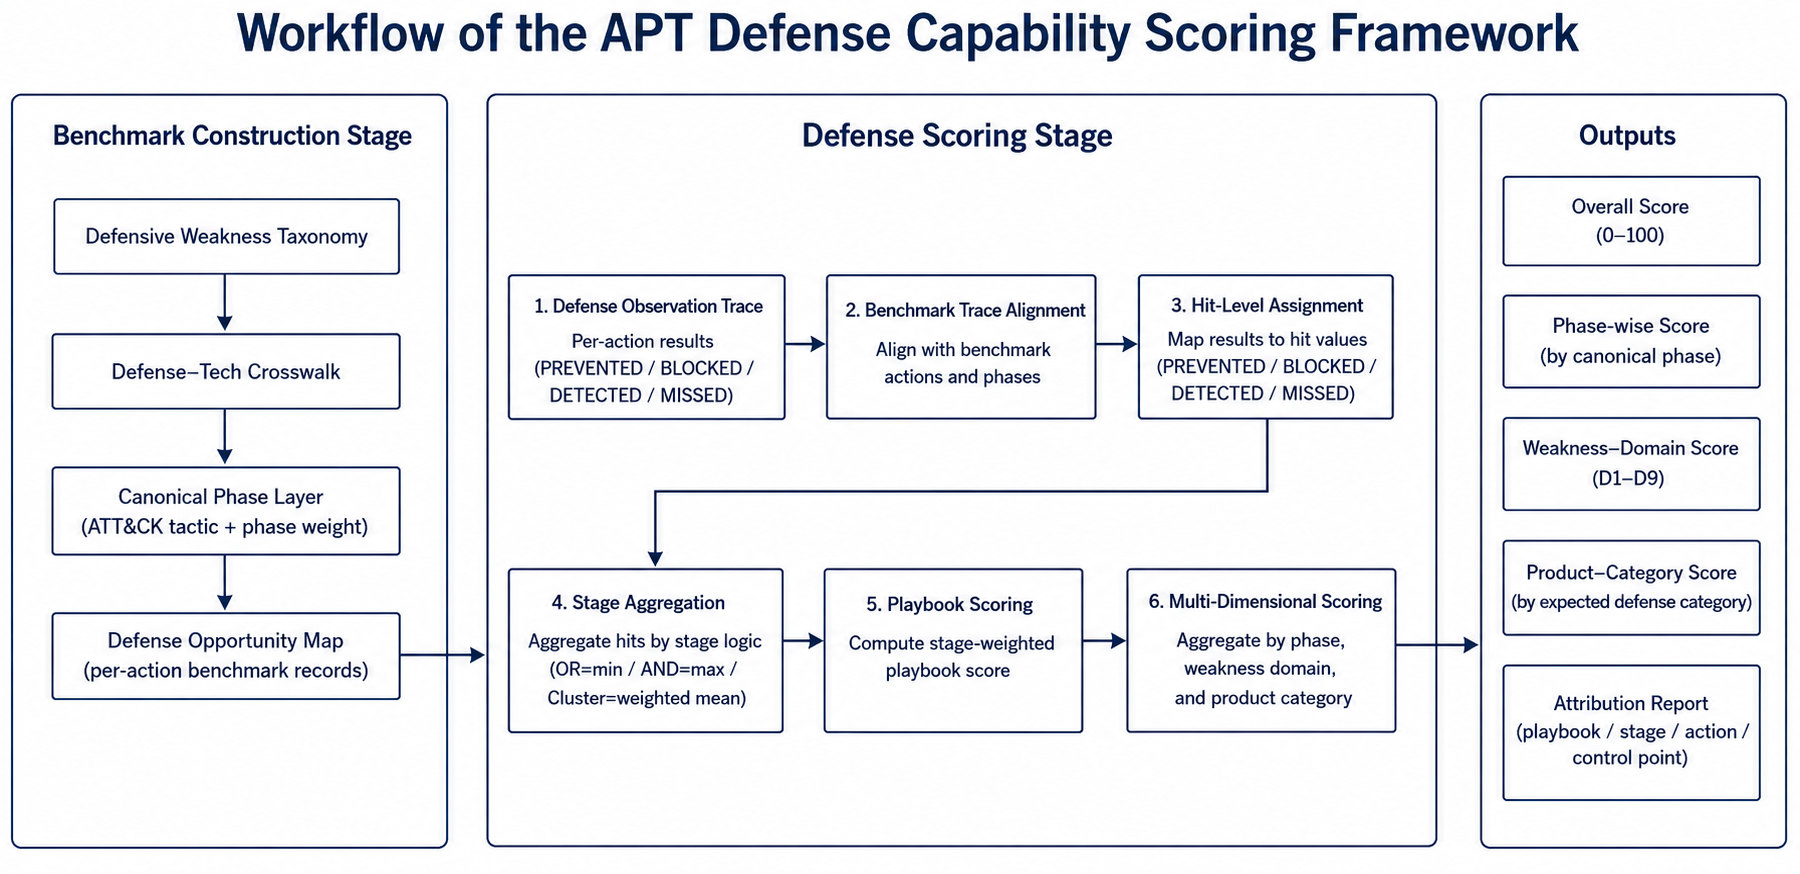
\includegraphics[width=0.95\textwidth]{figs/workflow.png}
  \caption{Workflow of the APT defense capability scoring framework.}
  \Description{Workflow of the proposed APT defense capability scoring framework, including benchmark construction, defense scoring, and score reporting.}
  \label{fig:methodology}
\end{figure*}


\subsection{Overview}
\label{subsec:methodology-overview}

The  framework converts multi-stage APT playbooks and action-level defense observations into interpretable defense capability scores. Its purpose is not only to record whether an attack step was detected or blocked, but also to explain why the step should have been stopped: which victim-side control point first failed, which defense product categories were expected to cover that weakness, and whether the evaluated defenses actually prevented, blocked, or detected the action.

Fig.~\ref{fig:methodology} illustrates the overall workflow. The process has three components: benchmark construction, defense scoring, and score reporting. During benchmark construction, raw APT playbook actions are annotated using a control-point attribution schema. Each action is mapped to the victim-side control point that first failed and is most relevant for repair. The annotated actions are then enriched with canonical attack phases, control-point-to-defense mappings, expected defense product categories, confidence labels, and stage aggregation semantics. The output of this step is a defense opportunity map, where each action is represented as a scoring-ready record.

During defense scoring, the evaluated system provides action-level observation results. Each observation is aligned with its corresponding action record in the defense opportunity map and translated into one of four hit levels: \texttt{PREVENTED}, \texttt{BLOCKED}, \texttt{DETECTED}, or \texttt{MISSED}. These levels capture different degrees of defensive success, from  prevention to complete miss. The scoring engine then aggregates action-level hit values into stage-level and playbook-level scores using the predefined aggregation semantics and canonical phase weights.

The final output is not a single  score. The framework reports an overall defense capability score together with phase scores, control-point domain scores, product category scores, and action level attribution reports. As a result, the score can be traced back to specific playbooks, stages, actions, and failed control points, which directly supports stage aware and attribution driven APT defense evaluation.



\subsection{Defensive Weakness Attribution}
\label{subsec:defensive-weakness-attribution}

We first map each attack action to the victim-side control point that first failed and is most relevant for repair. A control point refers to a defensive mechanism, configuration, policy, or operational process that can be evaluated and remediated independently. In this sense, a successful attack action indicates that a victim-side control was absent, misconfigured, bypassed, or insufficiently enforced.

This scope excludes actions that do not correspond to a directly repairable control point on the victim side. Pre-compromise reconnaissance, attacker-side infrastructure preparation, and similar external prerequisite activities are retained for playbook completeness, but they are not included in primary weakness statistics or attribution-based scoring unless a concrete victim-side control failure can be identified.

This attribution step is necessary because an ATT\&CK label tells us what the attacker did, but it does not tell us which defense failed. The same ATT\&CK technique may be enabled by different weaknesses in different environments. For example, a credential-related action may result from weak password policy, missing multi-factor authentication, exposed remote login services, insufficient credential storage protection, or successful phishing. These cases may share similar attack labels, but they imply different repair actions. Therefore, we interpret each action from the defender's perspective: given this action, which control point should be treated as the primary failure to repair?

Following this view, we use a structured control-point schema to organize recurring victim-side failures. The schema is not organized as an attack sequence. Instead, it separates defensive failures along four design dimensions: security function, architectural location, defensive lifecycle phase, and trust source. Security function distinguishes failures in identity, authorization, execution control, communication protection, and data protection. Architectural location separates externally exposed entry points from internal control failures. Defensive lifecycle phase separates prevention-oriented controls from observability, response, and resilience controls. Trust source captures weaknesses introduced through externally supplied inputs, such as phishing messages, malicious documents, third-party collaboration, and supply-chain entry points.

The schema contains nine top-level control-point domains and 94 fourth-level leaves. The top-level domains provide stable categories for attribution and reporting, while the leaf nodes capture more specific repair targets. In other words, the domains support interpretable scoring, and the leaves provide the operational granularity needed for remediation.

\begin{table}[t]
\centering
\caption{Top-level control-point domains.}
\label{tab:control-point-domains}
\begin{tabular}{p{0.12\columnwidth}p{0.76\columnwidth}}
\hline
Domain & Scope \\
\hline
D1 & Identity, credential, and trust-root failures \\
D2 & Authorization, isolation, and boundary-control failures \\
D3 & Execution, host, and runtime-protection failures \\
D4 & External exposure and remote-entry failures \\
D5 & Communication and protocol-design failures \\
D6 & Data protection, cryptographic-material, and recovery failures \\
D7 & Observability, detection, and response failures \\
D8 & External trust-input failures \\
D9 & Availability and resilience failures \\
\hline
\end{tabular}
\end{table}

Each in-scope action is assigned exactly one primary weakness leaf. This single-label rule keeps later scoring traceable. If a single action had multiple primary attributions, the same failure could be counted several times, and score loss could not be traced to a clear remediation target. To keep attribution consistent, the schema relies on explicit boundary rules and a primary-attribution decision principle: if only one control point could be repaired, the selected leaf should be the one whose repair would most directly prevent or disrupt the action.

Some actions still involve more than one relevant weakness. Secondary weakness tags are used to record such supporting conditions, including dual-control dependencies and entry--root-cause splits. These tags help explain attack chains, but they are not counted as primary attribution results and do not replace the primary leaf used for scoring.

In summary, defensive weakness attribution converts raw attack actions into repair-oriented control-point failures. This attributed action set then becomes the basis for the next steps of the methodology: canonical phase assignment, defense opportunity mapping, and stage-aware scoring.









\subsection{Benchmark Construction}
\label{subsec:benchmark-construction}
After attributing defensive weaknesses, the next step is to convert the attributed playbook actions into benchmark records that can be used for scoring. The attribution result alone is not sufficient for scoring: it tells us which control point failed, but it does not yet specify the attack stage, the expected defense product categories, or the aggregation semantics used later by the scoring engine. Benchmark construction adds these labels without changing the primary attribution result.

The benchmark construction process has three components. First, each action is mapped to a canonical attack phase using ATT\&CK. Second, each control-point leaf is mapped to the defense product categories that are expected to address it. Third, the enhanced action log is written into the defense opportunity map, which will serve as direct input to the scoring phase.

\subsubsection{Canonical Phase Assignment}
The attribution domains describe where the victim-side defense failed, rather than when the action occurs in the attack chain. However, scoring requires stage information because blocking an early-stage action and detecting a late-stage action should not have the same defensive value. Therefore, we add a separate canonical phase layer.

For each action, the framework assigns a canonical phase based on its ATT\&CK technique. We use the ATT\&CK Enterprise tactics as the standard phase vocabulary. Some ATT\&CK techniques can be associated with multiple tactics. We resolve this ambiguity using a predefined technique-to-phase mapping. Each technique is mapped to a single canonical phase before scoring, and this mapping remains fixed during defense scoring. Each technique is mapped to a single canonical phase before scoring, and this mapping remains fixed during defense scoring. Stage-level phases are then derived from the action-level phases, for example by majority voting among the actions in the same playbook stage. This phase assignment is an additional benchmark field; It does not change the control-point attribution described in the previous subsection.

The canonical phase field is later used by the scoring model to apply phase weights. The basic intuition is that earlier interruption has higher defensive value, while late-stage detection provides less benefit because the attacker has already progressed through much of the playbook.

\subsubsection{Defense-Category Mapping}
The primary weakness leaf identifies the failed control point, but a scoring benchmark also needs to know which type of defense product should be expected to address that failure. For this purpose, we build a defense-category mapping between control-point leaves and defense product categories.

Each fourth-level leaf is mapped to two sets of defense categories. The first set is the primary defense category set, which contains product types that should directly prevent or block the corresponding weakness if deployed and configured correctly. The second set is the compensating defense category set, which contains product types that may detect, mitigate, or partially compensate for the weakness, but are not the most direct repair target.

For example, a brute-force action attributed to weak password and anti-brute-force policy is primarily related to identity and access management, while privileged access management or log monitoring may provide compensating support. Similarly, a C2 communication action attributed to missing egress proxy enforcement may be primarily related to network access control or next-generation firewall capabilities, while SIEM or IDS may provide secondary visibility. This mapping allows later scoring to evaluate a product only against the actions that fall within its expected coverage set, rather than applying the same action set to all product categories.

\subsubsection{Defense Opportunity Map}
The final output of benchmark construction is the defense opportunity map. Each record in the map corresponds to one attack action and combines the information needed for scoring: the playbook identifier, stage number, action description, ATT\&CK technique, primary control-point leaf, top-level domain, canonical phase, expected defense categories, confidence label, and stage aggregation semantics.

The opportunity map keeps the primary attribution unique, but it also records additional defense opportunities when they are available. In particular, secondary weakness tags can be expanded into additional leaves and defense categories. This design preserves the repair-oriented primary attribution while still allowing the benchmark to represent layered defense opportunities.


The opportunity map also records the aggregation semantics used for each playbook stage. These semantics specify how the action-level hit values within a stage should be combined during scoring. For example, a stage may represent alternative attack paths, sequentially required actions, or a loose cluster of related actions. The detailed aggregation rules are defined in the scoring model.

Table~\ref{tab:opportunity-record-fields} summarizes the main fields used in the defense opportunity map.

\begin{table}[t]
\centering
\caption{Main fields in a defense opportunity record.}
\label{tab:opportunity-record-fields}
\begin{tabular}{p{0.30\columnwidth}p{0.58\columnwidth}}
\hline
Field & Meaning \\
\hline
playbook, stage, action & Identifier of the attack action in the playbook \\
attack\_id & ATT\&CK technique or sub-technique identifier \\
primary\_leaf & First-failed control-point leaf used for primary attribution \\
primary\_domain & Top-level control-point domain of the primary leaf \\
canonical\_phase & Standard attack phase used for phase-aware scoring \\
primary\_defense & Product categories expected to directly address the weakness \\
compensating\_defense & Product categories that may provide secondary detection or mitigation \\
confidence & Confidence of the primary attribution \\
stage\_logic & Aggregation semantics used later at the stage level \\
\hline
\end{tabular}
\end{table}

Through these steps, benchmark construction turns attributed attack actions into structured defense opportunities. The resulting records connect four pieces of information that are required for scoring: what the attacker did, which victim-side control point first failed, which defense categories were expected to cover the action, and how the action should contribute to stage-level aggregation.


\subsection{Defense Result Alignment}
\label{subsec:defense-result-alignment}
After the benchmark records are constructed, the evaluated defense system provides action-level observation results. Each observation describes how the defense system responded to a specific attack action in the playbook. The purpose of defense result alignment is to match these observations with the corresponding records in the defense opportunity map and convert them into normalized hit values for scoring.

We represent the defense observation trace as a set of action-level records. Each record contains the playbook identifier, the stage number, the action field used in the benchmark, and the observed result. Each defense observation is matched to the action record in the defense opportunity map with the same playbook identifier, stage number, and action field. After alignment, the observed result is associated with the action's control-point attribution, canonical phase, expected defense categories, confidence label, and stage aggregation semantics.

Actions without a matched defense observation are treated as missed actions. Under this rule, an action receives a positive hit value only when the evaluated defense system reports that it was prevented, blocked, or detected. Otherwise, the action is treated as \texttt{MISSED}. It also keeps the benchmark comparable across different defense systems: every system is evaluated against the same set of benchmark actions, and missing observations are interpreted as lack of demonstrated coverage.

Each matched observation is then converted into one of four hit levels. \texttt{PREVENTED} denotes architectural prevention, where the attack path is removed before the action can be attempted. \texttt{BLOCKED} denotes real-time interruption, where the action is attempted but stopped by the defense system. \texttt{DETECTED} denotes successful observation or alerting without stopping the action itself. \texttt{MISSED} denotes the absence of prevention, blocking, or detection. These levels are mapped to numerical hit values used by the scoring model.

\begin{table}[t]
\centering
\caption{Defense observation results and hit values.}
\label{tab:hit-levels}
\begin{tabular}{p{0.24\columnwidth}p{0.14\columnwidth}p{0.50\columnwidth}}
\hline
Result & Hit & Meaning \\
\hline
\texttt{PREVENTED} & 1.0 & The attack path is architecturally removed before the action can occur. \\
\texttt{BLOCKED} & 0.9 & The action is attempted but synchronously interrupted by the defense system. \\
\texttt{DETECTED} & 0.5 & The action is observed or alerted, but not stopped. \\
\texttt{MISSED} & 0.0 & The action is neither prevented, blocked, nor detected. \\
\hline
\end{tabular}
\end{table}

The distinction between \texttt{PREVENTED} and \texttt{BLOCKED} is important. Prevention means that the attack path is unavailable by design, such as when an egress policy makes an unauthorized destination unreachable. Blocking means that the action is observed and interrupted during execution, such as when an endpoint product terminates a malicious process. Both are stronger than detection-only outcomes, but prevention is assigned a slightly higher hit value because it does not depend on runtime recognition of the specific attack instance.

This alignment step produces a unified action-level scoring input. Each benchmark action is associated with both an expected defense opportunity and an observed defense result. 





\subsection{Stage-Aware Scoring Model}
\label{subsec:stage-aware-scoring}
After defense result alignment, each benchmark action has an action-level hit value and a set of benchmark metadata, including its canonical phase, attribution confidence, and stage aggregation semantics. The scoring model uses these fields to compute defense scores at three levels: action, stage, and playbook. The main design principle is to separate defense quality from stage importance. The stage score measures how well the defense performed within a stage, while the stage weight determines how much that stage contributes to the playbook-level score.

Let $a$ denote an attack action. Its hit value $h(a) \in [0,1]$ is obtained from the aligned defense result described in the previous subsection. The action weight $w(a)$ is defined as
\[
w(a) = W_{\mathrm{phase}}(\phi(a)) \cdot C_{\mathrm{conf}}(\gamma(a)),
\]
where $\phi(a)$ is the canonical phase assigned to action $a$, $W_{\mathrm{phase}}$ is the phase-weight function, $\gamma(a)$ is the attribution confidence label, and $C_{\mathrm{conf}}$ is the confidence factor. In our benchmark, the confidence factor reduces the contribution of actions whose attribution is less certain. For example, high-, medium-, and low-confidence actions can be assigned factors of $1.0$, $0.8$, and $0.5$, respectively.

For a playbook stage $s$, let $A_s$ be the set of actions in that stage. The stage score $S_s$ is computed according to the aggregation semantics of the stage. We use three aggregation types: OR, AND, and Cluster.

For an OR stage, the attacker only needs one action in the stage to succeed in order to proceed. Therefore, the defense must block all actions in the stage. The stage score is defined as
\[
S_s = \min_{a \in A_s} h(a).
\]
This reflects the weakest-link constraint: if any action is missed, the stage is considered poorly defended.

For an AND stage, the attacker needs all actions in the stage to succeed in order to complete the stage objective. Therefore, blocking any one required action can disrupt the stage. The stage score is defined as
\[
S_s = \max_{a \in A_s} h(a).
\]
This reflects the strongest defensive interruption within the stage.

For a Cluster stage, the actions do not have a strong logical dependency. They are treated as a group of related behaviors rather than as strict alternatives or strict requirements. The stage score is computed as a weighted average:
\[
S_s =
\frac{\sum_{a \in A_s} h(a) w(a)}
     {\sum_{a \in A_s} w(a)}.
\]
In this case, actions with higher phase importance or higher attribution confidence contribute more to the stage score.

The stage weight is computed separately from the stage score:
\[
W_s = \sum_{a \in A_s} w(a).
\]
This separation avoids mixing the quality of defense within a stage with the importance of that stage in the overall playbook. In particular, OR and AND stage scores are not weighted internally, because their semantics are determined by the attacker's path structure. The weights are used when aggregating stages into a playbook score.

For a playbook $P$ with stages $S(P)$, the playbook-level score is
\[
\mathrm{Score}(P) =
\frac{\sum_{s \in S(P)} W_s S_s}
     {\sum_{s \in S(P)} W_s}.
\]
The overall defense capability score is then computed by aggregating the scores over all evaluated playbooks:
\[
\mathrm{Score}_{\mathrm{overall}} =
\frac{1}{|\mathcal{P}|}
\sum_{P \in \mathcal{P}} \mathrm{Score}(P),
\]
where $\mathcal{P}$ denotes the set of playbooks in the benchmark. This formulation keeps the final score traceable: a score loss can be traced back from the overall score to a playbook, then to a stage, and finally to the individual actions and control-point failures that caused the loss.


\subsection{Multi-Dimensional Score Outputs}
\label{subsec:multi-dimensional-outputs}

The scoring model does not treat the overall score as the only output. A single aggregate score can indicate whether a defense system performs well on average, but does not explain where the score is gained or lost. To support diagnosis and comparison, the framework reports scores from multiple perspectives: overall performance, attack phase, control-point domain, defense product category, and action-level attribution.

The overall score summarizes the performance of the evaluated defense system in all playbooks. It is useful as a compact indicator, but is not intended to be interpreted alone. The same overall score may result from different defense profiles. For example, one system may cover many attack actions but only detect them late, while another system may cover fewer actions but block them reliably within its expected scope. Therefore, the overall score is reported together with the decomposed outputs.

The phase wise score groups results by canonical attack phase. This view answers the question: at which attack phases does the defense system lose the most score? Since the scoring model assigns higher value to earlier interception, phase wise results help distinguish early stage blocking from late stage observation. This directly supports stage aware analysis of APT defense capability.

The control point domain score groups results by the primary victim side control point domain. This view answers a different question: which type of defensive control fails most often or contributes most to score loss? For example, a low score in an identity related domain points to weaknesses in credential and trust controls, while a low score in an observability related domain indicates insufficient detection or response. This decomposition turns an aggregate score into repair-oriented feedback.

The product category score evaluates performance within the expected coverage of each defense product category. For a product category $c$, let $A_c$ denote the set of actions whose defense opportunity records include $c$ as a primary or compensating defense category. The coverage of $c$ is the fraction of benchmark actions that fall into this expected coverage set:
\[
\mathrm{Coverage}(c) = \frac{|A_c|}{|\mathcal{A}|},
\]
where $\mathcal{A}$ is the set of benchmark actions. The hit rate of $c$ is computed only within its coverage set:
\[
\mathrm{HitRate}(c) =
\frac{\sum_{a \in A_c} \tilde{h}_c(a)}
     {|A_c|}.
\]
Here, $\tilde{h}_c(a)$ is the hit value credited to category $c$. Primary defense matches receive full hit credit, while compensating defense matches may receive discounted credit because they detect or mitigate a weakness but do not directly eliminate the failed control point.

Reporting both coverage and hit rate is important. Coverage describes how much of the benchmark a product category is expected to address. Hit rate describes how well it performs within that expected scope. A product with narrow coverage but high hit rate has a different defense profile from a product with broad coverage but low hit rate, even if their aggregate scores are similar.

Finally, the framework produces an action level attribution report. For each score loss, the report retains the playbook, stage, action, ATT\&CK technique, canonical phase, primary control point leaf, defense categories, and observed result. This report provides the trace from aggregate score back to concrete attack actions and failed control points. As a result, the output can support both high level comparison and detailed remediation analysis.

\subsection{Prototype Method Validation}
\label{subsec:prototype-method-validation}

The preceding subsections define the attribution schema, benchmark construction process, result alignment procedure, scoring model, and multi-dimensional outputs. Before applying the framework to real defense-system replay experiments, we perform a set of prototype validation experiments on the benchmark and scoring infrastructure. These experiments do not evaluate a deployed defense product. Instead, they test whether the proposed methodological components are reproducible, whether the control-point--to--defense mapping is reasonable, and whether the scoring engine behaves correctly under boundary and parameter-variation cases.

First, we evaluate the reproducibility of defensive weakness attribution through a pilot inter-rater reliability study. A stratified sample of 50 ATT\&CK techniques and sub-techniques was independently labeled by two annotators using the same coding guide. Agreement was measured at multiple levels, including scope decision, top-level domain, leaf-level attribution, confidence label, mapping method, and secondary weakness tag. Table~\ref{tab:method-irr} summarizes the results.

\begin{table}[t]
\centering
\caption{Prototype validation of defensive weakness attribution.}
\label{tab:method-irr}
\begin{tabular}{p{0.36\columnwidth}p{0.18\columnwidth}p{0.18\columnwidth}p{0.20\columnwidth}}
\hline
Field & Agreement & $\kappa$ & Interpretation \\
\hline
Scope & 100.0\% & 1.000 & Almost perfect \\
L1 domain & 96.0\% & 0.953 & Almost perfect \\
L4 leaf & 86.0\% & 0.856 & Almost perfect \\
Confidence & 82.0\% & 0.679 & Substantial \\
Mapping method & 82.0\% & 0.687 & Substantial \\
Secondary tag & 66.0\% & 0.173 & Slight \\
\hline
\end{tabular}
\end{table}

The result shows that the primary attribution levels are reproducible in the pilot setting. The high agreement at the L1 and L4 levels indicates that the main control-point attribution can be applied consistently. In contrast, the secondary tag has much lower agreement, so it is retained as qualitative chain-context information rather than as a primary quantitative scoring field.

Second, we validate the defense-category mapping used by the Defense--Tech Crosswalk. The external validity check compares the crosswalk categories with the dataset's native control labels. Among 1,733 comparable actions, the two sources agree on 1,297 actions, giving an agreement rate of 74.8\%. We also perform an internal consistency check in which an independent annotator maps a stratified sample of 35 leaves to the 29 defense categories without seeing the existing crosswalk. Table~\ref{tab:method-crosswalk-validation} summarizes these checks.

\begin{table}[t]
\centering
\caption{Prototype validation of defense-category mapping.}
\label{tab:method-crosswalk-validation}
\begin{tabular}{p{0.42\columnwidth}p{0.44\columnwidth}}
\hline
Validation item & Result \\
\hline
External agreement with native control labels & 74.8\% (1,297 / 1,733 actions) \\
Highest category agreement & DLP 96.4\%, NET 93.6\%, EGW 90.3\% \\
Endpoint-category agreement & AV 73.5\%, EDR 71.9\% \\
Primary defense internal agreement & 97.1\% (34 / 35 leaves), $\kappa=0.485$ \\
Compensating defense internal agreement & 45.7\% (16 / 35 leaves), $\kappa=-0.094$ \\
\hline
\end{tabular}
\end{table}

These results suggest that the primary defense mapping is stable enough to support product-category scoring. The lower consistency for compensating defenses indicates that compensating coverage is less sharply defined than primary coverage. Therefore, compensating matches are treated as partial credit and should be interpreted more cautiously.

Third, we check the mathematical behavior of the scoring model using synthetic coverage traces. These traces are not real defense experiments; they are boundary and coverage simulations. A perfect-defense trace assigns \texttt{PREVENTED} to every benchmark action, and a no-defense trace assigns \texttt{MISSED} to every action. Two idealized product-category traces simulate systems that block all actions in their expected EDR or NGFW/NET primary coverage. Table~\ref{tab:method-coverage-simulation} reports the resulting scores.

\begin{table}[t]
\centering
\caption{Prototype scoring checks with synthetic coverage traces.}
\label{tab:method-coverage-simulation}
\begin{tabular}{p{0.26\columnwidth}p{0.52\columnwidth}p{0.12\columnwidth}}
\hline
Simulation & Configuration & Score \\
\hline
Perfect & All actions are \texttt{PREVENTED} & 100.00 \\
None & All actions are \texttt{MISSED} & 0.00 \\
Ideal EDR & EDR primary coverage $\rightarrow$ \texttt{BLOCKED} & 44.40 \\
Ideal NGFW & NGFW/NET primary coverage $\rightarrow$ \texttt{BLOCKED} & 24.93 \\
\hline
\end{tabular}
\end{table}

The perfect and none traces verify the expected upper and lower bounds of the scoring engine. The ideal EDR and ideal NGFW simulations show that a single product category cannot cover the whole benchmark even when it performs perfectly within its expected scope. This result reflects the multi-stage and multi-control nature of APT defense rather than the performance of a specific commercial product.

Finally, we test the robustness of the scoring results under reasonable parameter and aggregation variations. We vary phase weights, confidence factors, and compensating-defense discounts, and we also compare alternative aggregation choices for discovery-heavy Cluster stages and playbook-level aggregation. Table~\ref{tab:method-robustness} summarizes the main results.

\begin{table}[t]
\centering
\caption{Sensitivity and aggregation robustness checks.}
\label{tab:method-robustness}
\begin{tabular}{p{0.45\columnwidth}p{0.43\columnwidth}}
\hline
Check & Result \\
\hline
Perfect / none under all parameter settings & 100 / 0 in all configurations \\
EDR score range & 43.41--46.67 \\
NGFW score range & 23.62--27.57 \\
EDR/NGFW ratio range & 1.57--1.94 \\
Discovery-dominated Cluster alternative & Maximum score delta 1.07 \\
Action-count weighted playbook aggregation & Maximum score delta 0.78 \\
\hline
\end{tabular}
\end{table}

The sensitivity analysis shows that the boundary behavior of the scoring model remains stable across parameter settings, and the relative ordering between the idealized EDR and NGFW traces does not change. The aggregation robustness checks also show limited score variation under alternative but reasonable aggregation choices. These results support the use of the proposed scoring model as a stable prototype benchmark infrastructure. The later evaluation section will use real defense-system observations to test how deployed defenses perform under this methodology.








